\chapter{Scala} \label{Scala}
Scala on staattisesti tyypitetty moniparadigmainen käännettävä ohjelmointikieli, joka yhdistää funktionaalisen ohjelmoinnin ja olio-ohjelmoinnin ominaisuuksia. Scala on korkean tason kieli ja sen syntaksi on kompaktia ja eleganttia. Scalan kääntäjä ja tyyppijärjestelmä takaavat tyyppiturvallisuuden kääntämisen aikana muutamaa poikkeusta lukuunottamatta. Scala-koodi on tarkoitettu käännettäväksi Javan tavukoodiksi, ja se mahdollistaa Java-kirjastojen käyttämisen suoraan Scalasta. Tavukoodia ajetaan Javan virtuaalikoneessa (JVM). Tässä tutkielmassa tarkastellaan Scalan versiota 2.12.10.
\cite[Introduction]{tourOfScala}
\cite[Luku 2]{prorgrammingInScala3rd}


\section{Muuttujat} \label{Muuttujat}
Scalassa on tavallisten muuttujien lisäksi vakioita, jotka ovat muuttujia, joiden arvoa ei alustuksen jälkeen voi muuttaa. Vakion määrittelyyn käytetään avainsanaa \code{val} ja muuttujan määrittelyyn \code{var}. Funktionaalisessa Scalassa käytetään pääasiassa \code{val}-avainsanalla määriteltyjä muuttujia, ja imperatiivisessa tyylissä voidaan käyttää molempia.

Muuttujan nimen jälkeen määritellään muuttujan tyyppi, joka erotetaan muuttujan nimesta kaksoispisteellä. Esimerkiksi \code{val x: Int = 1} alustaa kokonaislukuvakion x, jonka arvo on 1. Muuttujan tyyppimäärittelyn voi jättää myös kirjoittamatta, sillä Scala-kääntäjä osaa yleensä päätellä muuttujan tyypin asetetun arvon perusteella. Edellisen esimerkin voi siis halutessaan kirjoittaa muodossa \code{val x = 1}, ja Scala osaa päätellä muuttujan olevan tyypiltään kokonaisluku.
\cite[Basics]{tourOfScala}

Muuttujat ovat myös staattisesti tyypitettyjä, joten muuttujan tyyppi ei voi muuttua ajon aikana. Scalassa myös funktiot ovat arvoja, joten niitä voidaan sijoittaa muuttujiin. Esimerkiksi \code{val add1 = (x: Int) => x + 1} luo \textit{funktioliteraalin} ja sijoittaa sen muuttujaan nimeltä add1. Funktioita käsitellään tarkemmin luvussa \ref{MetoditJaFunktiot}.
\cite[Luku 1]{prorgrammingInScala3rd}


\section{Tietotyypit}
Scala on puhtaasti oliokieli, eli kaikki arvot ja muuttujat ovat olioita. Jokainen Scalan tietotyyppi perii luokan \code{Any} ja luokka \code{Nothing} on jokaisen tietotyypin alaluokka. Scalassa luokka voi olla arvoluokka tai viiteluokka. Arvoluokat perivät luokan \code{AnyVal} ja niihin ei voi sijoittaa null-arvoa. Viiteluokat perivät luokan \code{AnyRef}, joka on tyyppialias Javan luokalle \code{Object}. Jokaisen viiteluokan alaluokka on \code{Null}. Tietotyyppien hierarkia on kuvattu kuvassa \ref{tyyppihierarkia}.
\cite[Luku 5]{prorgrammingInScala3rd}

\begin{figure}[h]
    \centering 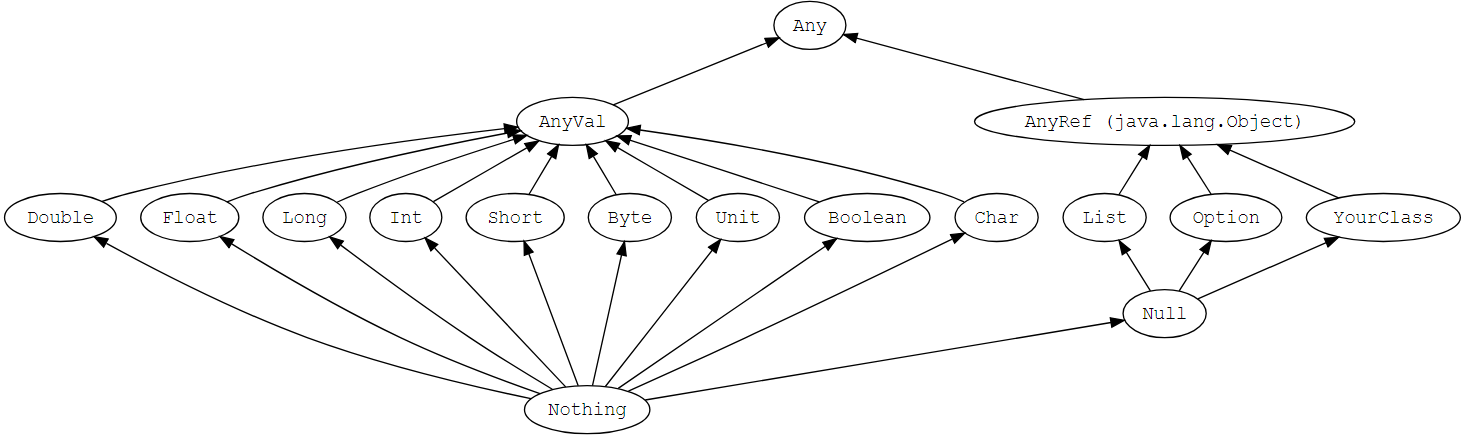
\includegraphics[width=1\textwidth]{kuvat/typehierarchy}
    \caption{Scalan luokkahierarkia}
    \label{tyyppihierarkia}
\end{figure}

Alkeistietotyyppejä kuvaavat arvoluokat \code{Byte}, \code{Short}, \code{Int}, \code{Long}, \code{Char}, \code{Float}, \code{Double}, \code{Boolean} ja \code{Unit}. Kaikki paitsi \code{Unit} vastaavat Javan vastaavia kääreluokkia. \code{Unit} on erityinen tietotyyppi, joka kuvastaa funktion tyhjää paluuarvoa. Sen voi ajatella vastaavan Javan void-avainsanaa. Merkkijonoja Scalassa kuvaa tietotyyppi \code{String}, joka on tyyppialias Javan merkkijonoa kuvaavalle tietotyypille.
\cite[Luku 5]{prorgrammingInScala3rd}

Scalan alkeistietotyypit muutetaan käännösvaiheessa primitiivityypeiksi, esimerkiksi Scalan \code{Int} käännetään 32-bittiseksi sanaksi, aivan kuten Javan \code{int}. Tämä takaa yhteensopivuuden Java-kirjastojen kanssa. Se parantaa myös suorituskykyä, sillä primitiiviarvolle ei tarvitse allokoida muistia ajon aikana.
\cite[Luku 6]{prorgrammingInScala3rd}


\section{Kontrollirakenteet}

\subsection{Ehtolauseet}
Ehtolauseita kirjoitetaan Scalassa \textit{if/else}-lausekkeiden avulla. Lauseketta voi käyttää imperatiiviseen tyyliin eli jos ehto arvioituu todeksi, suoritetaan if-lohko, muuten else-lohko.
\begin{lstlisting}
    val x = true
    if (x) {
        println("True")
    } else {
        println("False")
    }
    // Tulostaa "True"
\end{lstlisting}
Scalan if-lausekkeella on myös arvo, eli if-lauseke palauttaa arvon. Arvon palauttavaa if-lauseketta voidaan käyttää myös funktionaalisessa ohjelmoinnissa. Esimerkiksi \codebl{val y = if (x >= 0) \"positive\" else \"negative\"} asettaa muuttujan \code{y} arvoksi joko merkkijonon "positive" tai "negative", riippuen muuttujan \code{x} arvosta. Huomattavaa on myös, että if-lauseke voidaan kirjoittaa yhdelle riville ilman aaltosulkeita. 
\cite[Luku 2.1]{scalaForTheImpatient}
        
\subsection{Silmukat}
Silmukoita Scalassa on kolmenlaisia: \code{while}, \code{do} ja \code{for}. While-silmukka suorittaa sitä seuraavaa lohkoa 0-n kertaa, kunnes annettu ehto arvioituu epätodeksi. Do-silmukka toimii vastaavalla tavalla, mutta sitä suoritetaan 1-n kertaa.
\begin{lstlisting}
    val x = false
		while (x)
			println("while")
		
		do
			println("do")
        while (x)
\end{lstlisting}
Yllä oleva esimerkki ei suorita while-silmukkaa kertaakaan, ja do-silmukan kerran.
\cite[Luku 2.5]{scalaForTheImpatient}

Scalan \code{for}-lauseke on monipuolisempi kuin monissa muissa kielissä. Sitä voi käyttää perinteiseen tapaan silmukkana, jolloin for-lausekkeen \textit{generaattori} antaa määriteltyjä arvoja yksi kerrallaan muuttujan \code{i} kautta. Lauseketta voidaan käyttää myös usean generaattorin kanssa ja arvoja voidaan suodattaa lausekkeen sisällä. Kuten if-lauseke, myös for-lauseke voi palauttaa arvon. Seuraavaksi esimerkki kummastakin käyttötavasta.
\begin{lstlisting}
    for (i <- 1 to 10)
        println(i)
\end{lstlisting}
Silmukkana lauseketta voi käyttää yllä olevan esimerkin tapaan tulostamaan kaikki numerot yhdestä kymmeneen.
\begin{lstlisting}
    val res = for {
        x <- 1 to 10
        if x % 2 == 0
    } yield (x * 2) // Vector(4, 8, 12, 16, 20)
\end{lstlisting}
Yllä olevassa esimerkissä luodaan kokonaisnumerovektori yhdestä kymmeneen, suodatetaan parilliset arvot, palautetaan jäljelle jäääneet arvot kahdella kerrottuna ja asetetaan palautettu vektori muuttujaan \code{res}. Tälläinen \code{for}-lauseke on yleinen funktionaalisessa Scalassa.
\cite[Luku 2.6]{scalaForTheImpatient}


\section{Metodit ja funktiot} \label{MetoditJaFunktiot}
Jokainen operaatio Scalassa on metodikutsu. Myös tavanomaiset aritmeettiset operaattorit on toteutettu metodikutsuina. Esimerkiksi kahden kokonaisluvun yhteenlasku \code{1 + 2} on lyhyempi versio metodikutsusta \code{1.+(2)}. Scalassa on mahdollista määritellä funktio kahdella tavalla: olion metodiksi tai funktioliteraaliksi. Metodi voidaan määritellä \code{def}-avainsanalla.
Scalassa funktio palauttaa automaattisesti viimeisen lausekkeensa arvon, joten \code{return}-avainsanan käyttö on vapaaehtoista ja sitä käytetään vain harvoin.
\cite[Luku 1.4]{scalaForTheImpatient}
\cite[Basics]{tourOfScala}

\subsection{Funktioliteraalit}
Funktioliteraali on funktio, jota käsitellään kuten mitä tahansa muuttujaa. Yleensä funktioliteraali sijoitetaan muuttujaan tai annetaan parametriksi toiselle funktiolle. Kuten muillakin muuttujilla, funktioilla ja metodeilla on Scalassa aina tyyppi. Tyypin voi määritellä eksplisiittisesti, mutta monesti Scala osaa päätellä funktion tyypin.
Seuraavassa esimerkissä määritellään kummallakin tavoilla funktio, joka kertoo onko parametrina annettu kokonaisluku parillinen. Funktion tyyppi on siis \code{Int => Boolean}.
\cite[Luku 8]{prorgrammingInScala3rd}
\begin{lstlisting}
    def isEven1(x: Int): Boolean = x % 2 == 0
    val isEven2: (Int => Boolean) = x => x % 2 == 0
\end{lstlisting}

\subsection{Korkeamman asteen funktiot}
Funktio voi ottaa parametriksi toisen funktion tai palauttaa funktion. Tälläisiä funktioita kutsutaan \textit{korkeamman asteen funktioiksi}. Korkeamman asteen funktiot ovat yksi funktionaalisen ohjelmoinnin kulmakivistä. Seuraavassa esitellään korkeamman asteen funktio, joka ottaa parametrina kokonaisluvun sekä funktion kokonaisluvusta kokonaislukuu, ja palauttaa kutsuu tätä funktiota parametrin kokonaisluvulle.
\begin{lstlisting}
    def mapValue(v: Int, m: Int => Int): Int = m(v)
    
    def double(x: Int): Int = x * 2
    
    mapValue(2, double)
    mapValue(2, _ * 3)
\end{lstlisting}
Kuten yllä olevasta esimerkistä huomataan, annetaan \code{double}-funktio parametrinä ihan kuten mikä tahansa muukin muuttuja. Esimerkin viimeisellä rivillä käytetään funktioliteraalia \code{_ * 3}, joka on lyhyempi muoto funktioliteraalille \code{x => x * 3}.
\cite[Luku 12]{scalaForTheImpatient}


\section{Luokat ja oliot} \label{LuokatJaOliot}
Scalassa on useita erilaisia luokka- ja oliotyyppejä sekä tapoja luoda instansseja luokista. Tässä luvussa esitellään pääpiirteittäin erilaiset luokkatyypit.

\subsection{Class} \label{class}
Luokka voidaan määritellä Scalassa \code{class}-avainsanalla. Luokka voi olla tyhjä tai se voi sisältää metodeita ja muuttujia. Luokasta luodaan instanssi \code{new}-avainsanalla. Luokan sisältämät kentät voidaan määritellä konstruktorissa heti luokan nimen jälkeen suluissa. Konstruktorissa määritellyt kentät ovat oletuksena \code{private val}. Luokasta saadaan uusi instanssi \code{new}-avainsanan avulla. Ihmistä kuvaava luokka ja instanssi voidaan määritellä seuraavalla tavalla:
\begin{lstlisting}
    class Person(val name: String, var age: Int) {
        def isAdult = age >= 18
    }
    val p = new Person("Matti", 30)
\end{lstlisting}
Luokassa Person on kaksi kenttää: julkinen muuttumaton kenttä nimi ja julkinen muutettava ikä. Lisäksi luokassa on metodi, joka kertoo onko henkilö täysi-ikäinen.
\cite[Classes]{tourOfScala}


\subsection{Case class} \label{caseclass}
Scalassa on myös erityisiä case-luokkia, joita käytetään yleensä kuvaamaan muuttumatonta dataa. Case-luokka määritellään kuten tavallinen luokka, mutta konstruktorissa määriteltävät kentät ovat oletuksena \code{public val}. Case-luokkaan voidaan määräitellä metodeita samoin kuin tavalliseenkin luokkaan. Case-luokan instanssia luotaessa ei tarvitse käyttää \code{new}-avainsanaa. Puhelinmallia kuvaava case-luokka ja instanssi voidaan määritellä seuraavalla tavalla:
\begin{lstlisting}
    case class Phone(brand: String, model: String)
    val p = Phone("Google", "Pixel4")
\end{lstlisting}
Scala-kääntäjä lisää case-luokkiin \code{toString}-, \code{hashCode}-, \code{equals}- ja \code{copy}-metodeita oletustoteutuksilla. Lisäksi kääntäjä lisää \textit{kumppaniolioon} \code{apply}-tehdasmetodin, jonka avulla uusien instanssien luonti tapahtuu.
\cite[Luku 15]{prorgrammingInScala3rd}

Tavallisia luokkia käytetään varsinkin oliotyylisessä ohjelmoinnissa, kun taas case-luokat ovat käytössä erityisesti funktionaalisessa Scalassa, kun halutaan käyttää muuttumattomia olioita. Tavallisten luokkien ja case-luokkien yhtäsuuruusvertailut eroavat toisistaan merkittävästi. Tavallisia luokkia verrataan viittauksen mukaan, eli osoittaako viittaus samaan olioon JVM:ssä. Case-luokkien yhtäsuuruutta verrataan olion kenttien arvon mukaan.
\cite[Luku 15]{prorgrammingInScala3rd}

\subsection{Singleton-oliot} \label{singleton-oliot}
Useat muut oliokielet tarjoavat mahdollisuuden kirjoittaa staattisia luokkia tai staattisia kenttiä luokkiin. Scalassa tälläistä staattisuutta ei ole, vaan vastaava toiminnallisuus mahdollistetaan erityisien \textit{singleton}-olioiden kautta. Singleton-oliosta on ajon aikana olemassa vain yksi instanssi, ja Scala luo sen automaattisesti. Singleton-olion on mahdollista periä luokka. Viittaaminen olioon tapahtuu yksinkertaisesti olion nimellä.
\cite[Singleton objects]{tourOfScala}

Singleton-oliota voidaan kutsua myös kumppaniolioksi, jos se on määritelty saman nimisen luokan yhteydessä. Kumppanioliot näkevät ilmentymiensä yksityiset kentät, ja ilmentymät näkevät kumppaniolionsa yksityiset kentät. Luvun \ref{caseclass} Phone-luokalle voidaan luoda kumppaniolio seuraavalla tavalla:
\begin{lstlisting}
    object Phone {
        def iphone11 = new Phone("Apple", "iPhone 11")
    }
    val iphone = Phone.iphone11
\end{lstlisting}
Tässä tapauksessa kumppanioliossa on vain yksi metodi, jonka avulla voidaan luoda helposti instansseja.
\cite[Luku 4]{prorgrammingInScala3rd}


\subsection{Piirretyypit} \label{piirretyypit}
Piirretyyppejä käytetään Scalassa määrittelemään olioiden tarjoamien palveluiden rajapintoja ja mahdollistamaan ohjelmakoodin uudelleenkäytettävyyttä. Uusi piirretyyppi luodaan \code{trait}-avainsanalla. Piirretyyppien on myös sallittua periä toisia piirretyyppejä tai luokkia. Myös singleton-olioihin on mahdollista liittää piirretyyppejä. Piirretyypin voi ajatella olevan Javan rajapintaluokan ja abstraktin luokan yhdistelmä.
\cite[Luku 6 ja 12]{prorgrammingInScala3rd}

Piirretyypin jäseniksi voidaan määritellä metodeita tai muuttujia. Jäsenet voivat olla abstrakteja tai konkreetteja. Abstraktille jäsenelle tulee toteuttavan luokan tarjota toteutus, kun taas konkreettielle jäsenille ei. Yhdessä piirreluokassa voi olla sekä abstrakteja että konkreetteja jäseniä. Tietyissä erityistapauksissa metodi voidaan merkitä abstraktiksi, vaikka sille on annettu toteutus piirretyypissä.
\cite[Luku 10]{scalaForTheImpatient}
